 \documentclass{beamer}
%
% Choose how your presentation looks.
% For more themes, color themes and font themes, see:
% http://deic.uab.es/~iblanes/beamer_gallery/index_by_theme.html
%
\mode<presentation>
{
  \usetheme{Madrid}      % or try Darmstadt, Madrid, Warsaw, ...
  \usecolortheme{seahorse} % or try albatross, beaver, crane, ...
  \usefonttheme{serif}  % or try serif, structurebold, ...
  \setbeamertemplate{navigation symbols}{}
  \setbeamertemplate{caption}[numbered]
  \setbeamertemplate{itemize/enumerate body begin}{\large}
\setbeamertemplate{itemize/enumerate subbody begin}{\large}
\setbeamertemplate{itemize/enumerate subsubbody begin}{\large}

  \usepackage{amsmath}
  \usepackage{bm}
  \usepackage{subcaption}
  \usepackage{tcolorbox}
  \usepackage[export]{adjustbox}
  \tcbuselibrary{most}
  \usepackage{arydshln}
  \usepackage{tikz}
  \usetikzlibrary{plotmarks}
  \usepackage{pgfplots}
  \usepackage{booktabs}
\usepackage[inkscapeformat=png]{svg}
 %\usepackage{enumitem}
%\usepackage{enumerate}
  %\usepackage[shortlabels]{enumitem}
} 


\definecolor{myblue}{RGB}{65,105,225} 
\definecolor{myorange}{RGB}{250,190,0}

\setbeamercolor{structure}{fg=white,bg=myorange}
\setbeamercolor*{palette primary}{fg=myblue,bg=myorange}
\setbeamercolor*{palette secondary}{fg=white,bg=myblue}
\setbeamercolor*{palette tertiary}{bg=myblue,fg=white}
\setbeamercolor*{palette quaternary}{fg=white,bg=myorange!50}

\setbeamercolor{frametitle}{fg=black!90!myblue}

\setbeamercolor{section in head/foot}{fg=white,bg=myblue}
\setbeamercolor{author in head/foot}{fg=black,bg=myorange}
\setbeamercolor{title in head/foot}{fg=white,bg=myblue}

\setbeamertemplate{navigation symbols}{}

\setbeamertemplate{itemize/enumerate body begin}{\large}
\setbeamertemplate{itemize/enumerate subbody begin}{\large}


\defbeamertemplate*{headline}{mytheme}
{%
  \begin{beamercolorbox}[ht=2.25ex,dp=3.75ex]{section in head/foot}
    \insertnavigation{\paperwidth}
  \end{beamercolorbox}%
}%

\defbeamertemplate*{footline}{mytheme}
{
  \leavevmode%
  \hbox{%
  \begin{beamercolorbox}[wd=.5\paperwidth,ht=2.25ex,dp=1ex,right]{author in head/foot}%
    \usebeamerfont{author in head/foot}\insertshortauthor\hspace*{2em}
  \end{beamercolorbox}%
  \begin{beamercolorbox}[wd=.5\paperwidth,ht=2.25ex,dp=1ex,left]{title in head/foot}%
    \usebeamerfont{title in head/foot}\hspace*{2em}\insertshortsubtitle\hspace*{2em}
    \insertframenumber{} / \inserttotalframenumber
  \end{beamercolorbox}}%
  \vskip0pt%
}


\usepackage[greek,german,russian,french,english]{babel}
\usepackage[LAE,T1]{fontenc}
%\usepackage[utf8x]{inputenc}
\usepackage{xcolor}
\usepackage{xurl}
\usepackage{listings}
\usepackage{pgf}  
\usepackage{textpos}
\usepackage{tabulary}
\usepackage{scrextend}
\usepackage{hyperref}
\usepackage{setspace}
\usepackage{rotating}
\lstset
{
    language=[LaTeX]TeX,
    breaklines=true,
    basicstyle=\tt\scriptsize,
    %commentstyle=\color{green}
    keywordstyle=\color{blue},
    %stringstyle=\color{black}
    identifierstyle=\color{magenta},
}
\newcommand{\bftt}[1]{\textbf{\texttt{#1}}}
%\newcommand{\comment}[1]{{\color[HTML]{008080}\textit{\textbf{\texttt{#1}}}}}
\newcommand{\cmd}[1]{{\color[HTML]{008000}\bftt{#1}}}
\newcommand{\bs}{\char`\\}
\newcommand{\cmdbs}[1]{\cmd{\bs#1}}
\newcommand{\lcb}{\char '173}
\newcommand{\rcb}{\char '175}
\newcommand{\cmdbegin}[1]{\cmdbs{begin\lcb}\bftt{#1}\cmd{\rcb}}
\newcommand{\cmdend}[1]{\cmdbs{end\lcb}\bftt{#1}\cmd{\rcb}}

\newcommand{\wllogo}{\textbf{Overleaf}}

% this is where the example source files are loaded from
% do not include a trailing slash
\newcommand{\fileuri}{https://raw.githubusercontent.com/GiancarloSucci/UniBo.IDSEPC.A2022/main/A2022.IDSEPCLaTeX/}


\usepackage{stackengine}
\def\Ruble{\stackengine{.67ex}{%
  \stackengine{.48ex}{\textsf{P}}{\rule{.8ex}{.12ex}\kern.6ex}{O}{r}{F}{F}{L}%
  }{\rule{.8ex}{.12ex}\kern.6ex}{O}{r}{F}{F}{L}\kern-.1ex}



%----------------------------------------------------------------------------------------
%	TITLE PAGE
%----------------------------------------------------------------------------------------
\title[L07]{Artificial Intelligence, Blockchain, e Criptovalute nello Sviluppo Software \newline\newline
Lezione 9: Software as Story Telling} % The short title appears at the bottom of every slide, the full title is only on the title page

\author[{\tiny Giancarlo Succi }]{Giancarlo Succi\\\\ Dipartimento di Informatica -- Scienza e Ingegneria\\Universit\`{a} di Bologna\\
\bftt{g.succi@unibo.it}
} % Your name
\institute[unibo] % Your institution as it will appear on the bottom of every slide, may be shorthand to save space


\date{} % Date, can be changed to a custom date

\setbeamertemplate{navigation symbols}{}
\AtBeginSection[]
{
        \begin{frame}<beamer>{Outline}
                \tableofcontents[currentsection]
        \end{frame}
}
\begin{document}

\begin{frame}
\titlepage % Print the title page as the first slide

\end{frame}

%=============================================

\addtobeamertemplate{frametitle}{}{%
\begin{textblock*}{10mm}(-0.01mm,-0.95cm)

\includegraphics[width=0.9cm]{unibo-logo.png}
\end{textblock*}}

%=============================================

\begin{frame}
{\centerline{Content}}
       \begin{tabular}{lc}  
       \begin{tabular}{l}
             \parbox{0.4\linewidth}{%  change the parbox width as appropiate
             \begin{itemize}
                \item Story telling $\ldots{}$ why?
                \item Italo Calvino and his work
                \item The story telling in Calvino:
                \begin{itemize}
                    \item Lightness
                    \item Rapidity
                    \item Precision
                    \item Visibility
                    \item Multiplicity
                \end{itemize}
            \end{itemize}

             }
         \end{tabular} &
         \begin{tabular}{c}
           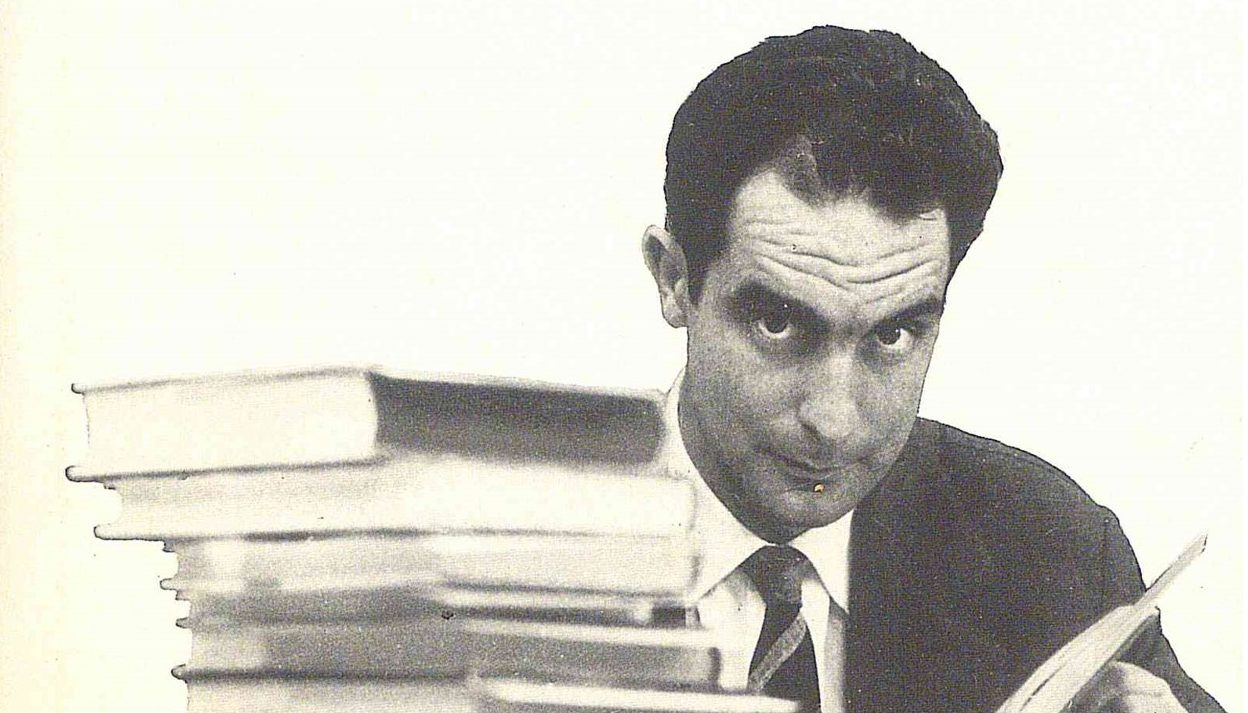
\includegraphics[width=.5\textwidth]{P2023.AIBCCSS.StoryTelling/Calvino5.jpg}
           \end{tabular}
       \end{tabular}
 \begin{center}
 \tiny  Source of this lecture: Paolo Ciancarini, Sergey Masyagin, and Giancarlo Succi. 2020. ``Software design as story telling: reflecting on the work of Italo Calvino.'' In Proceedings of the 2020 ACM SIGPLAN International Symposium on New Ideas, New Paradigms, and Reflections on Programming and Software (Onward! 2020). Association for Computing Machinery, New York, NY, USA, 195–208.\newline
 
 A video presentation of this material can be found at : \url{https://dl.acm.org/doi/abs/10.1145/3426428.3426925}

 \end{center}
\end{frame}

\begin{frame}
{\centerline{Story telling $\ldots{}$ why?}}

       \begin{tabular}{cl}  
         \begin{tabular}{c}
           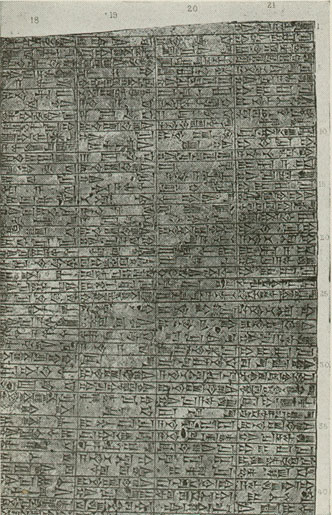
\includegraphics[width=.4\textwidth]{P2023.AIBCCSS.StoryTelling/CodeOfHammurabi.jpg}
           \end{tabular}
           & \begin{tabular}{l}
             \parbox{0.5\linewidth}{%  change the parbox width as appropiate
             \Large
             \begin{itemize}
                \item Software is about \textcolor{red}{\bf writing}
                \item \textcolor{gray}{Software is about writing} \textcolor{red}{\bf stories}
                \item Writing is about communicating desires, orders, memories, sequences of actions
            \end{itemize}

             }
         \end{tabular}
       \end{tabular}
\end{frame}



\begin{frame}
{\centerline{Cato}}

\begin{figure}[htp]
    \centering
     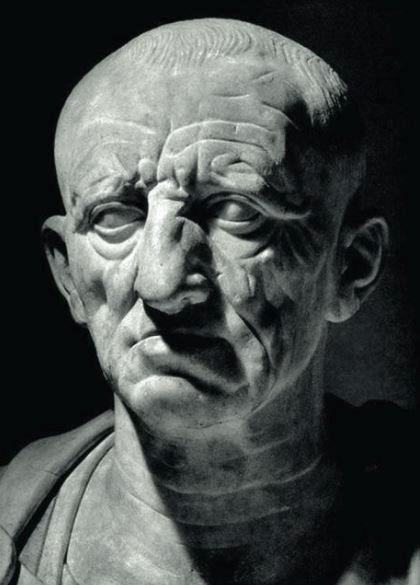
\includegraphics[width=.32\textwidth]{P2023.AIBCCSS.StoryTelling/CatoneIlCensore.jpg}
    \label{F:CatoneIlCensore}
\end{figure}

\begin{center}
    \Large{\textcolor{red}{Rem tene,} \textcolor{blue}{verba sequentur!}}\\
    \textit{Does it tell anything to us for writing software?}
\end{center}
\end{frame}



\begin{frame}
{\centerline{Cicero}}

       \begin{tabular}{cl}  
         \begin{tabular}{c}
           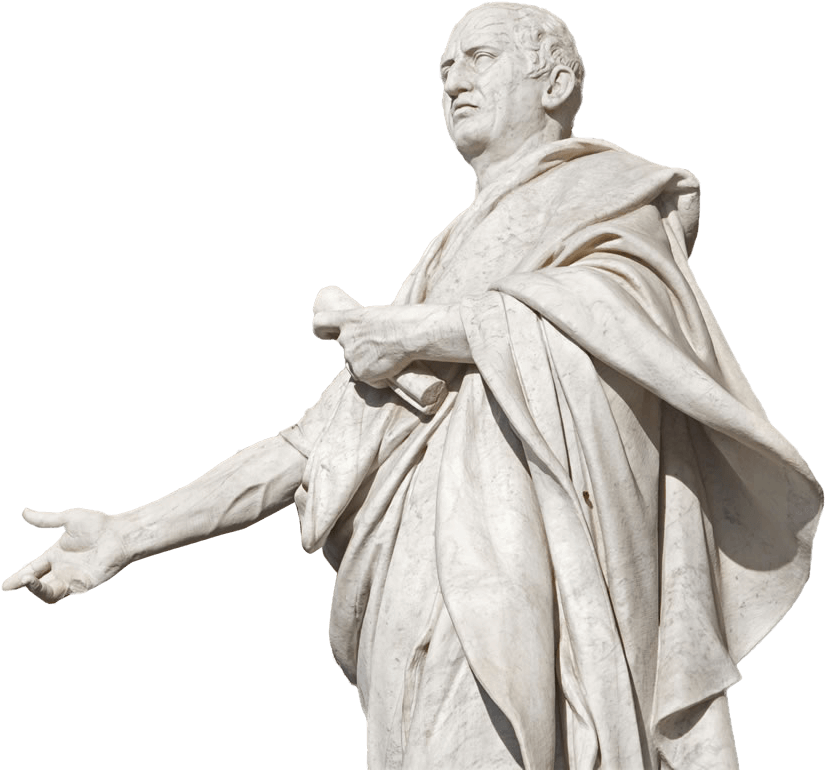
\includegraphics[width=.5\textwidth]{P2023.AIBCCSS.StoryTelling/Cicero.png}
           \end{tabular}
           & \begin{tabular}{l}
             \parbox{0.5\linewidth}{%  change the parbox width as appropiate
             \Large
             \begin{itemize}
                \item Inventio
                \item Dispositio
                \item Elocutio
                \item Memoria
                \item Actio
             \end{itemize}

            }
         \end{tabular}
       \end{tabular}

\end{frame}

\begin{frame}
{\centerline{Dante}}

       \begin{tabular}{cl}  
         \begin{tabular}{c}
           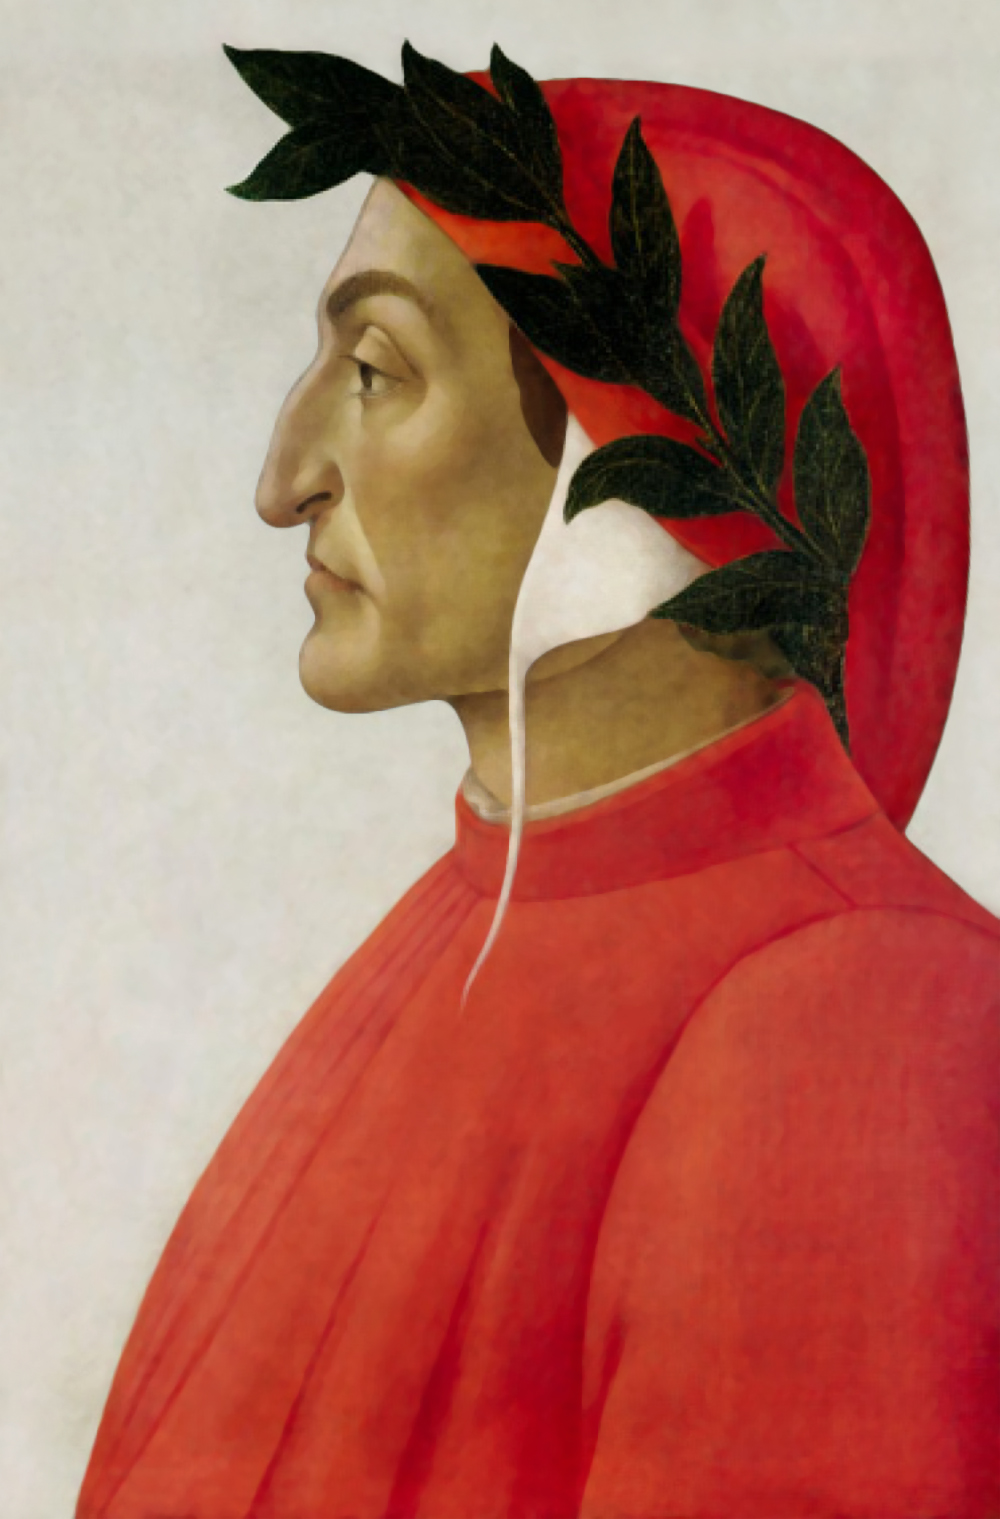
\includegraphics[width=.35\textwidth]{P2023.AIBCCSS.StoryTelling/Dante.jpg}
           \end{tabular}
           & \begin{tabular}{l}
             \parbox{0.6\linewidth}{%  change the parbox width as appropiate
            E io a lui: ``I' mi son un che, quando\\
            Amor mi spira, noto, \textcolor{red}{\bf e a quel modo}\\
            ch'e' ditta dentro vo significando.''
            }
         \end{tabular}
       \end{tabular}

\end{frame}

\begin{frame}
{\centerline{Lodovico Castelvetro}}

       \begin{tabular}{cl}  
         \begin{tabular}{c}
           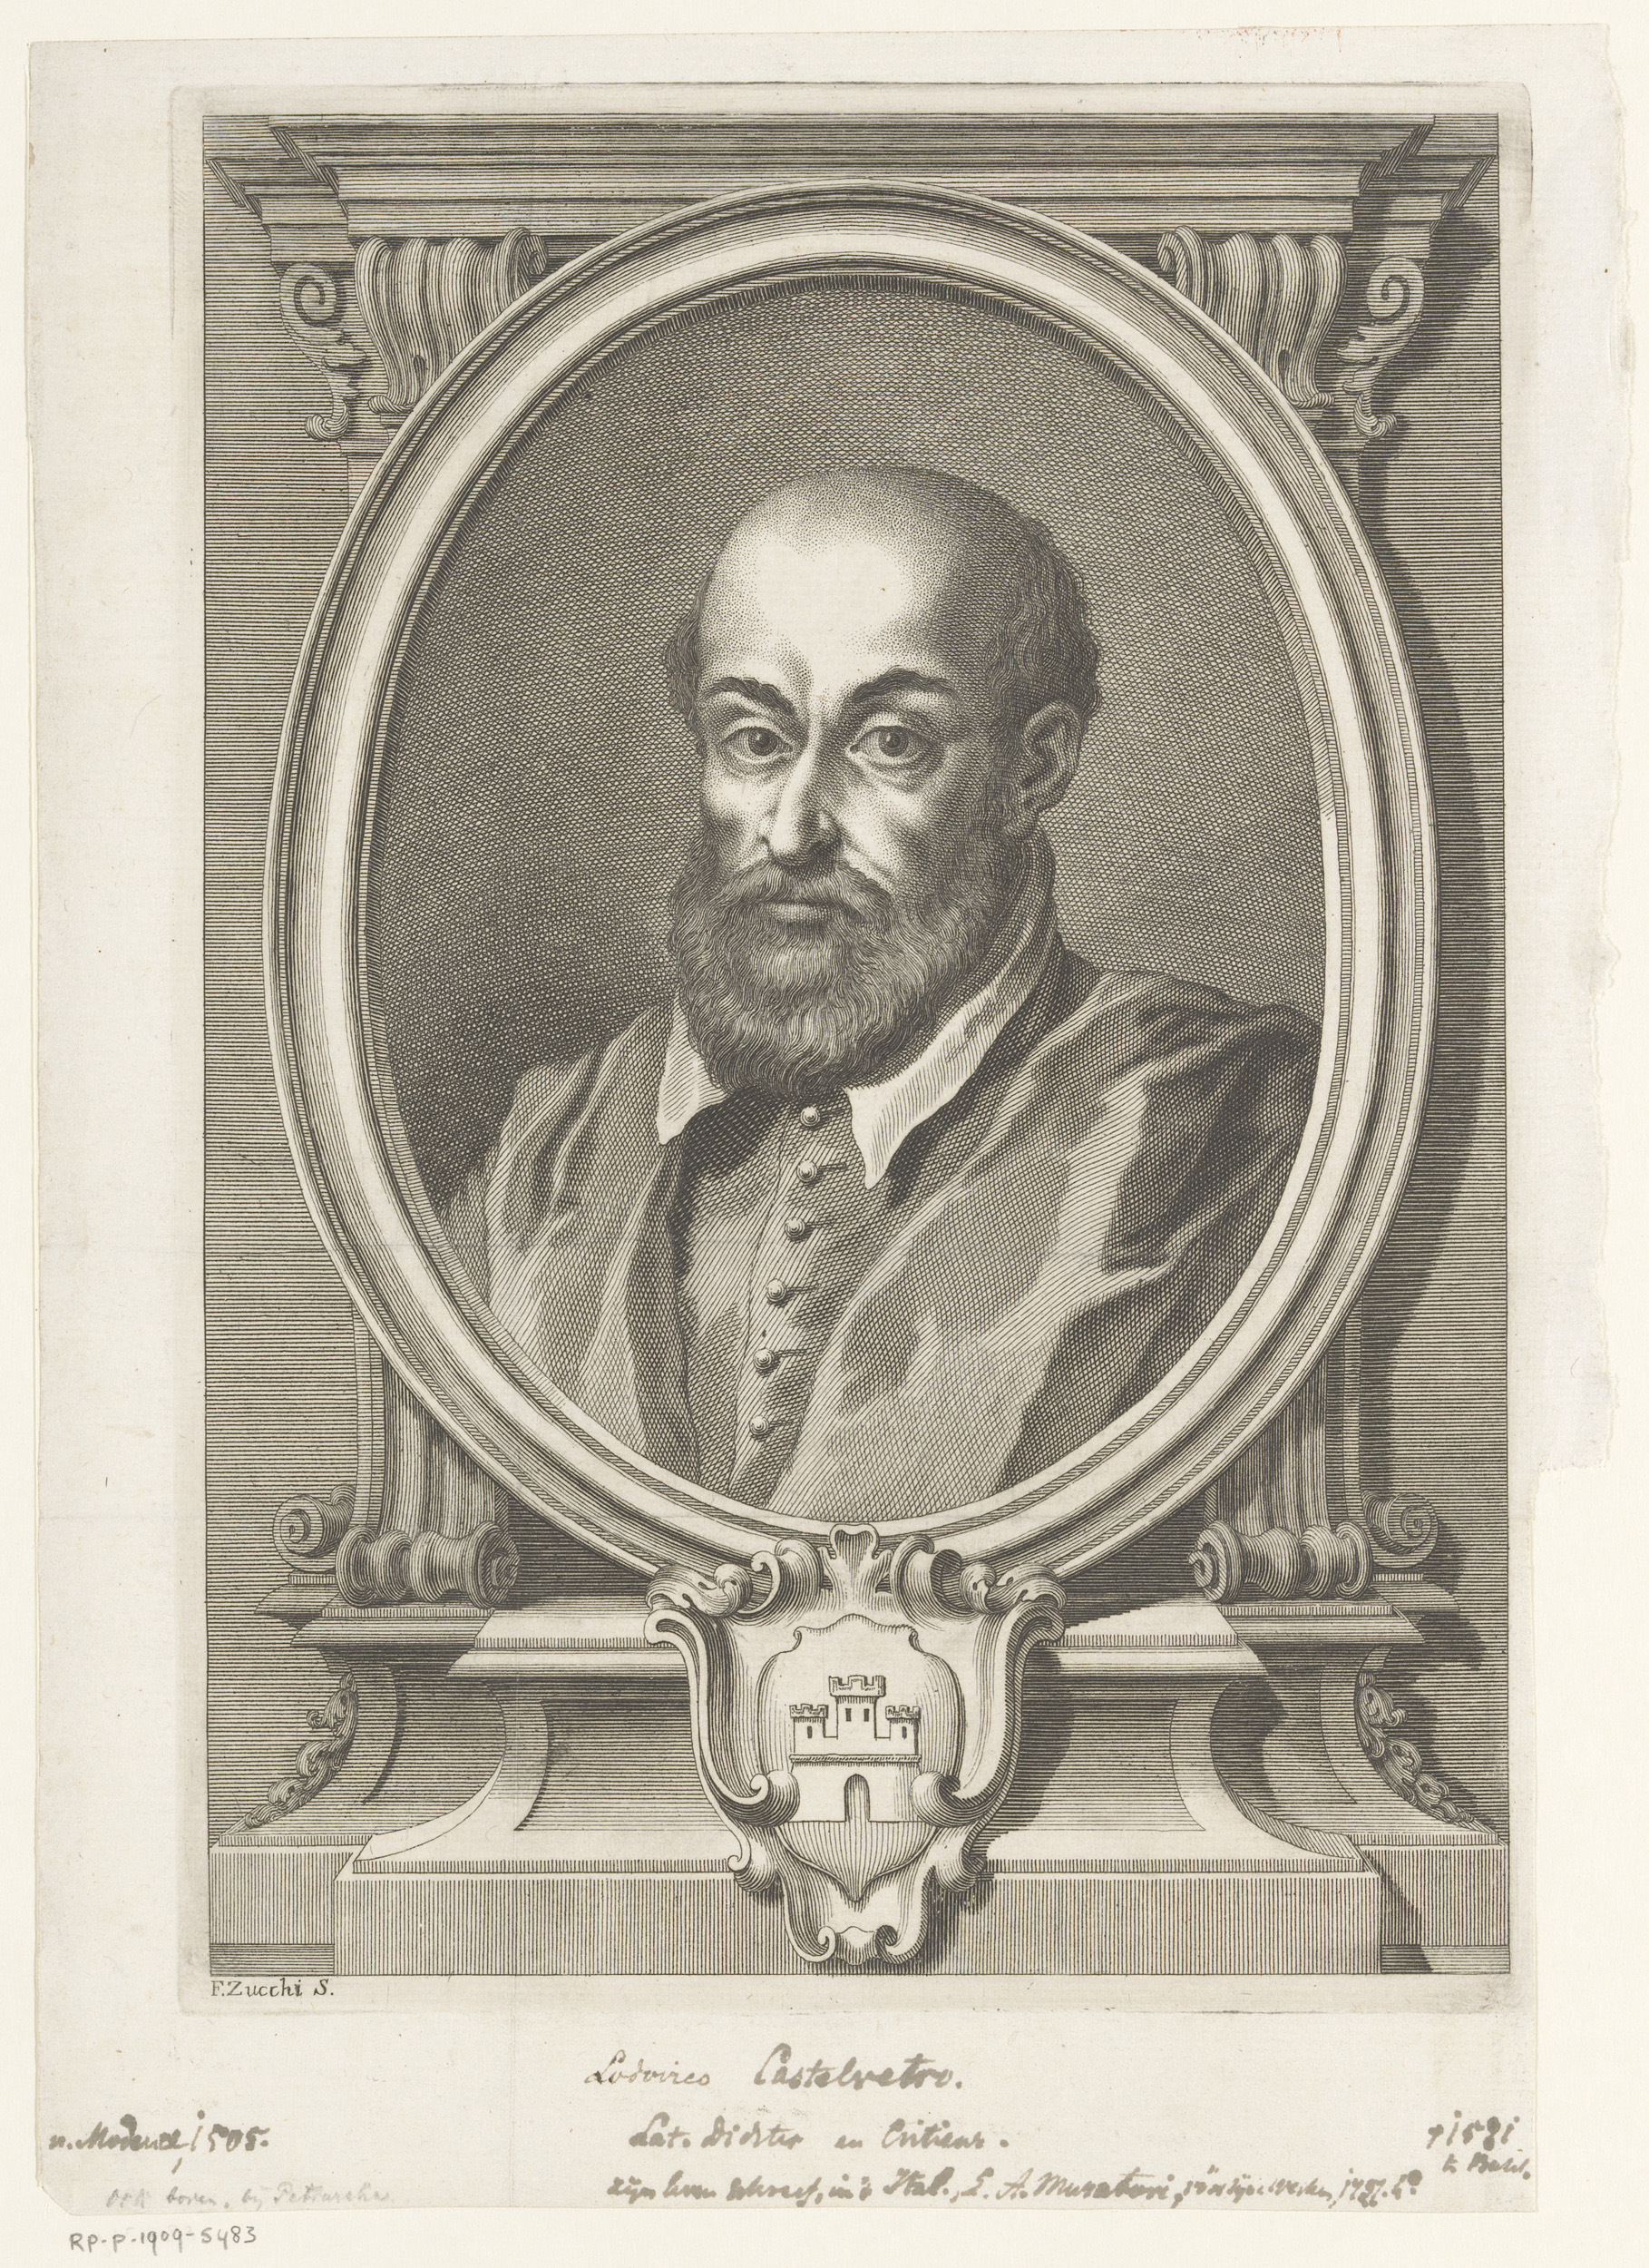
\includegraphics[width=.45\textwidth]{P2023.AIBCCSS.StoryTelling/LodovicoCastelvetro.jpg}
           \end{tabular}
           & \begin{tabular}{l}
              \parbox{0.45\linewidth}{%  change the parbox width as appropiate
              The facts presented in the play should $\ldots{}$
               \begin{itemize}
                \item \textcolor{red}{time}: $\ldots{}$ span typically one day;\\
                \item \textcolor{red}{place}: $\ldots{}$ occur in a limited location, usually one city;\\
                \item \textcolor{red}{action}: $\ldots{}$ refer usually to one single situation.\\
               \end{itemize}
               The \textcolor{blue}{three Aristotelian unities}! Don't they resemble modularity, cohesion, separation of concerns? 
             }
         \end{tabular}
       \end{tabular}

\end{frame}

\begin{frame}
{\centerline{Italo Calvino and his work}}

       \begin{tabular}{cl}  
         \begin{tabular}{c}
           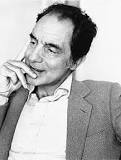
\includegraphics[width=.4\textwidth]{P2023.AIBCCSS.StoryTelling/Calvino.jpg}
           \end{tabular}
           & \begin{tabular}{l}
             \parbox{0.5\linewidth}{%  change the parbox width as appropiate
             \begin{itemize}
                \item Cuba, 1923 -- Italy 1985
                \item Italian, with international profile
                \item Writer, journalist, systemic
                \item Visitor of both Russia/USSR and USA
            \end{itemize}

             }
         \end{tabular}
       \end{tabular}

\end{frame}

\begin{frame}
{\centerline{Italo Calvino and his work}}

       \begin{tabular}{cl}  
         \begin{tabular}{c}
           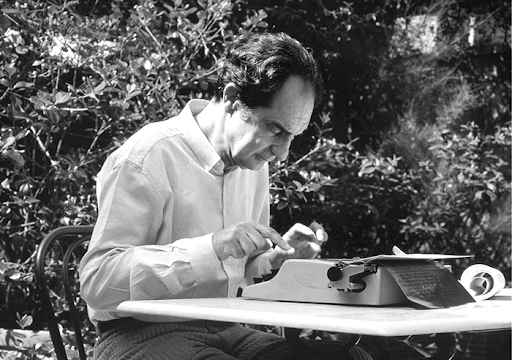
\includegraphics[width=.4\textwidth]{P2023.AIBCCSS.StoryTelling/Calvino2.png}
           \end{tabular}
           & \begin{tabular}{l}
             \parbox{0.5\linewidth}{%  change the parbox width as appropiate
             \begin{itemize}
                \item Inspired by cybernetics and informatics
                \item Even tried to build stories out of combinatorics of situations
                \item Huge attention to the semantics of the words and of the sentences as collections of words
            \end{itemize}

             }
         \end{tabular}
       \end{tabular}

\end{frame}


\begin{frame}
{\centerline{Italo Calvino and his work}}

       \begin{tabular}{cl}  
         \begin{tabular}{c}
           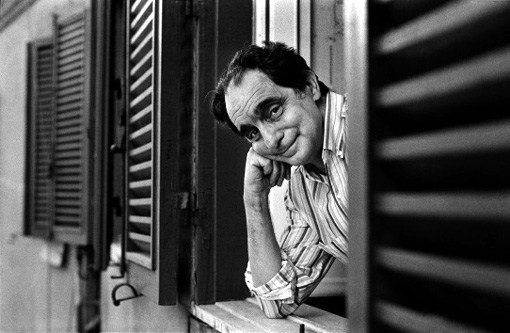
\includegraphics[width=.4\textwidth]{P2023.AIBCCSS.StoryTelling/Calvino3.jpg}
           \end{tabular}
           & \begin{tabular}{l}
             \parbox{0.5\linewidth}{%  change the parbox width as appropiate
             \begin{itemize}
                \item Wrote (without completing) ``Six Memos for the Next Millennium''
                \item  6 lectures given at Harvard (should have been)
                \item What the third millennium should learn from the second
            \end{itemize}

             }
         \end{tabular}
       \end{tabular}

\end{frame}

\begin{frame}
{\centerline{Italo Calvino and his work}}

       \begin{tabular}{cl}  
         \begin{tabular}{c}
           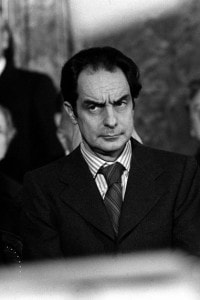
\includegraphics[width=.4\textwidth]{P2023.AIBCCSS.StoryTelling/Calvino4.jpg}
           \end{tabular}
           & \begin{tabular}{l}
             \parbox{0.5\linewidth}{%  change the parbox width as appropiate
             \begin{itemize}
                \item Lightness
                \item Rapidity
                \item Precision
                \item Visibility
                \item Multiplicity
                \item \textit{[ Coherence ]}
            \end{itemize}
            \vspace{1cm}
            Note: our own translation, not 100\% compliant with the ``usual.''
             }
         \end{tabular}
       \end{tabular}

\end{frame}


\begin{frame}
{\centerline{Agile Development as Storytelling}}

\begin{itemize}
\item Rooted in the Agile Manifesto \newline
\item Emphasis on people  \textcolor{blue}{interactions}, on  \textcolor{blue}{working code}, on  \textcolor{blue}{conversations} among stakeholders \newline
\item Requirements as user \textcolor{red}{stories} \newline
\item Metaphor, in the words of Kent Beck: ``The system metaphor is a \textcolor{red}{story} that everyone--customers, programmers, and managers--can \textcolor{red}{tell} about how the system works."
\end{itemize}

\end{frame}



\begin{frame}
{\centerline{Our goals}}
\begin{itemize}
\item \textcolor{blue}{Retrospective:} Further and deeper reflections on the \textcolor{red}{analogies between writing software and writing} 
\begin{itemize}
\item analysing how software engineers have come to similar conclusions as art critics
\end{itemize}
\vspace{0.5cm}
\item \textcolor{blue}{Ambition}: \textcolor{red}{Proposals of improvements} based on these reflections
\begin{itemize}
\item Calvino as 
\begin{itemize}
\item a case study and
\item a concrete reference.
\end{itemize}
\end{itemize}
\end{itemize}

\end{frame}


\begin{frame}
{\centerline{Lightness}}

\begin{itemize}
\item Two apparently contradicting aims of writers:
\begin{itemize}
\item to provide a \textcolor{red}{comprehensive description} of the world, and
\item to be \textcolor{red}{agile} in writing, \textcolor{blue}{easy to read}, \textcolor{orange}{lively}, \textcolor{cyan}{engaging}. 
\end{itemize}
\vspace{0.5cm}
\item Complexity is like \textcolor{red}{Medusa}: she attracts inexorably anyone trying to contemplate her. 
\begin{itemize}
\item Perseus kills her \textcolor{red}{cutting her head} looking at a reflection of it on a kind of mirror
\item Then, he does not throw the head away but he \textcolor{blue}{keeps it in a nice and honorable container} and uses it it as a weapon against his enemies.
\end{itemize}
\end{itemize}

\end{frame}

\begin{frame}
{\centerline{Lightness}}
\Large
\begin{tcolorbox}[fonttitle=\bfseries,nobeforeafter,center title,colback=yellow!5,colframe=yellow!40!black,title=Calvino]
    ``There is a \textcolor{olive}{lightness of thoughtfulness} and a \textcolor{blue}{lightness of levity}. \\
    
    The \textcolor{olive}{lightness of thoughtfulness} can make the \textcolor{blue}{lightness of levity} to appear \textcolor{red}{\bf heavy}."
\end{tcolorbox}

\end{frame}

\begin{frame}
{\centerline{Lightness in SW}}

\begin{figure}[htp]
    \centering
     
\includegraphics[width=.9\textwidth]{P2023.AIBCCSS.StoryTelling/EasyChangeBeck.png}
    \label{F:EasyChangeBeck}
\end{figure}

\end{frame}


\begin{frame}
{\centerline{Lightness in SW}}

\begin{figure}[htp]
    \centering
     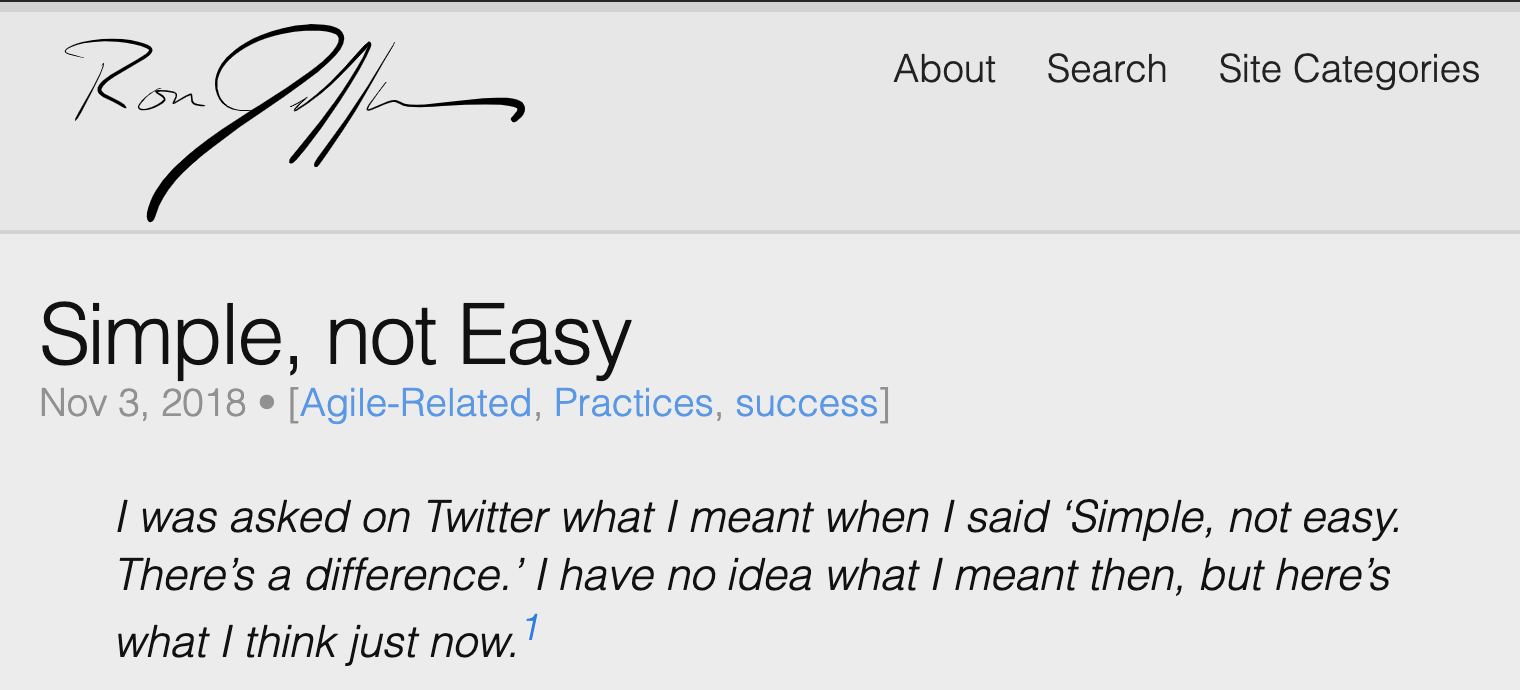
\includegraphics[width=.85\textwidth]{P2023.AIBCCSS.StoryTelling/EasyChangeJeffries.png}
    \label{F:EasyChangeJeffries}
\end{figure}
\vspace{-0.4cm}
\begin{tcolorbox}[colback=gray!5,colframe=gray!5]
\small
``But the quote – see, I came back – whatever its original context, refers to lots of things in Agile and in life. Scrum is simple; it isn’t easy. Exercise, diet: they’re simple, but not easy. Love is simple, but not easy.''
\begin{center}
    \tiny{From:  \url{https://ronjeffries.com/articles/018-01ff/simple-not-easy/}}
\end{center}
\end{tcolorbox}

\end{frame}


\begin{frame}
{\centerline{Lightness -- New perspectives}}

\begin{tcolorbox}[colback=yellow!5,colframe=yellow!40!black]
``The empty bucket, sign of deprivation, desire, and quest, which elevates you to a point where your humble prayer cannot any more be answered, paves the way for endless reflections.''
\end{tcolorbox}

\begin{itemize}
\item Lightness as \textcolor{red}{deprivation}
\item Understanding what \textcolor{red}{cannot be fully described} in writing
\item \textcolor{red}{Using an incomplete language} and then taking advantage of the incompleteness to hint at what it is impossible to express explicitly 
\item It could be an effective way to manage \textcolor{red}{uncertainty}, \textcolor{blue}{mutability}, and \textcolor{orange}{variability}.
\end{itemize}

\end{frame}


\begin{frame}
{\centerline{Rapidity}}

\begin{itemize}
\item Not a fast random movement but the result of competence, knowledge, and thinking
\item \textcolor{red}{Festina lente!}
\end{itemize}
\vspace{0.2cm}
\begin{tcolorbox}[colback=yellow!5,colframe=yellow!40!black]
``Among the multiple virtues of Chuang-Tzu there was the ability to draw. The king asked him to draw a crab. Chuang-Tzu replied that he needed 5 years and a villa with 12 servants. After five years the drawing was not yet started: `I need five more years' said Chuang-Tzu and the king accepted. \textcolor{blue}{At the end of the ten years Chuang-Tzu took the brush and with a single movement draw a crab, the \textbf{most perfect crab ever seen}}.''
\end{tcolorbox}

\end{frame}

\begin{frame}
{\centerline{Rapidity in SW}}

       \begin{tabular}{cl}  
         \begin{tabular}{c}
           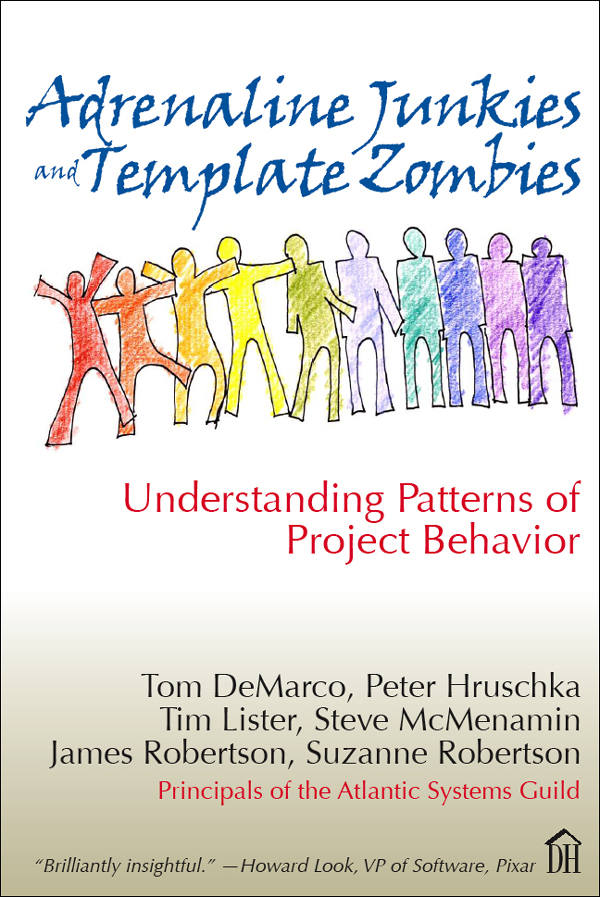
\includegraphics[width=.4\textwidth]{P2023.AIBCCSS.StoryTelling/AndrenalineJunkies.jpeg}
           \end{tabular}
           & \begin{tabular}{l}
             \parbox{0.5\linewidth}{%  change the parbox width as appropiate
             \begin{itemize}
                \item ``\textcolor{red}{Adrenaline Junkies}. The organization believes that frenzied activity is a sign of healthy productivity.''
                \item ``\textcolor{red}{Management By Mood Ring}. The manager reports status based on activities, effort, and enthusiasm of the team rather than on the risks, decisions, and issues facing the project.''
                \item $\ldots{}$

            \end{itemize}

             }
         \end{tabular}
       \end{tabular}

\end{frame}



\begin{frame}
{\centerline{Rapidity in SW}}

\begin{itemize}
 \item Also $\ldots{}$ Tom De Marco (2001) \textit{Slack: Getting Past Burn-out, Busywork, and the Myth of Total Efficiency,} Dorset House Publishing\vspace{0.3cm}
\item Kent Beck, Cynthia Andres (2004) \textit{Extreme Programming Explained: Embrace Change, Second Edition,} Addison Wesley \\
\begin{itemize}
\item ``Sometimes courage manifests as patience.
\item If you know there is a problem but you don’t know what it is, $\ldots{}$
\item $\ldots{}$ \textcolor{red}{it takes \textbf{courage} to wait} for the real problem to emerge distinctly.''
\end{itemize}
\end{itemize}

\end{frame}

\begin{frame}
{\centerline{More on Rapidity}}

\begin{itemize}
\item ``Mercury and Vulcan represent two inseparable and complementary vital functions: Mercury the syntony, that is, \textcolor{red}{the participation to the world around us}, and Vulcan the focus, \textcolor{blue}{the constructive concentration}.'' \vspace{0.2cm}
\item ``Around the \textcolor{cyan}{\textbf{magic object}} there is a force field that is the narration. We can say that the magic object makes explicit the connection between people and events. $\ldots{}$ And in a narration an object is always a magic object.''

\end{itemize}

\end{frame}

\begin{frame}
{\centerline{More on Rapidity in SW}}

\begin{figure}[htp]
    \centering
     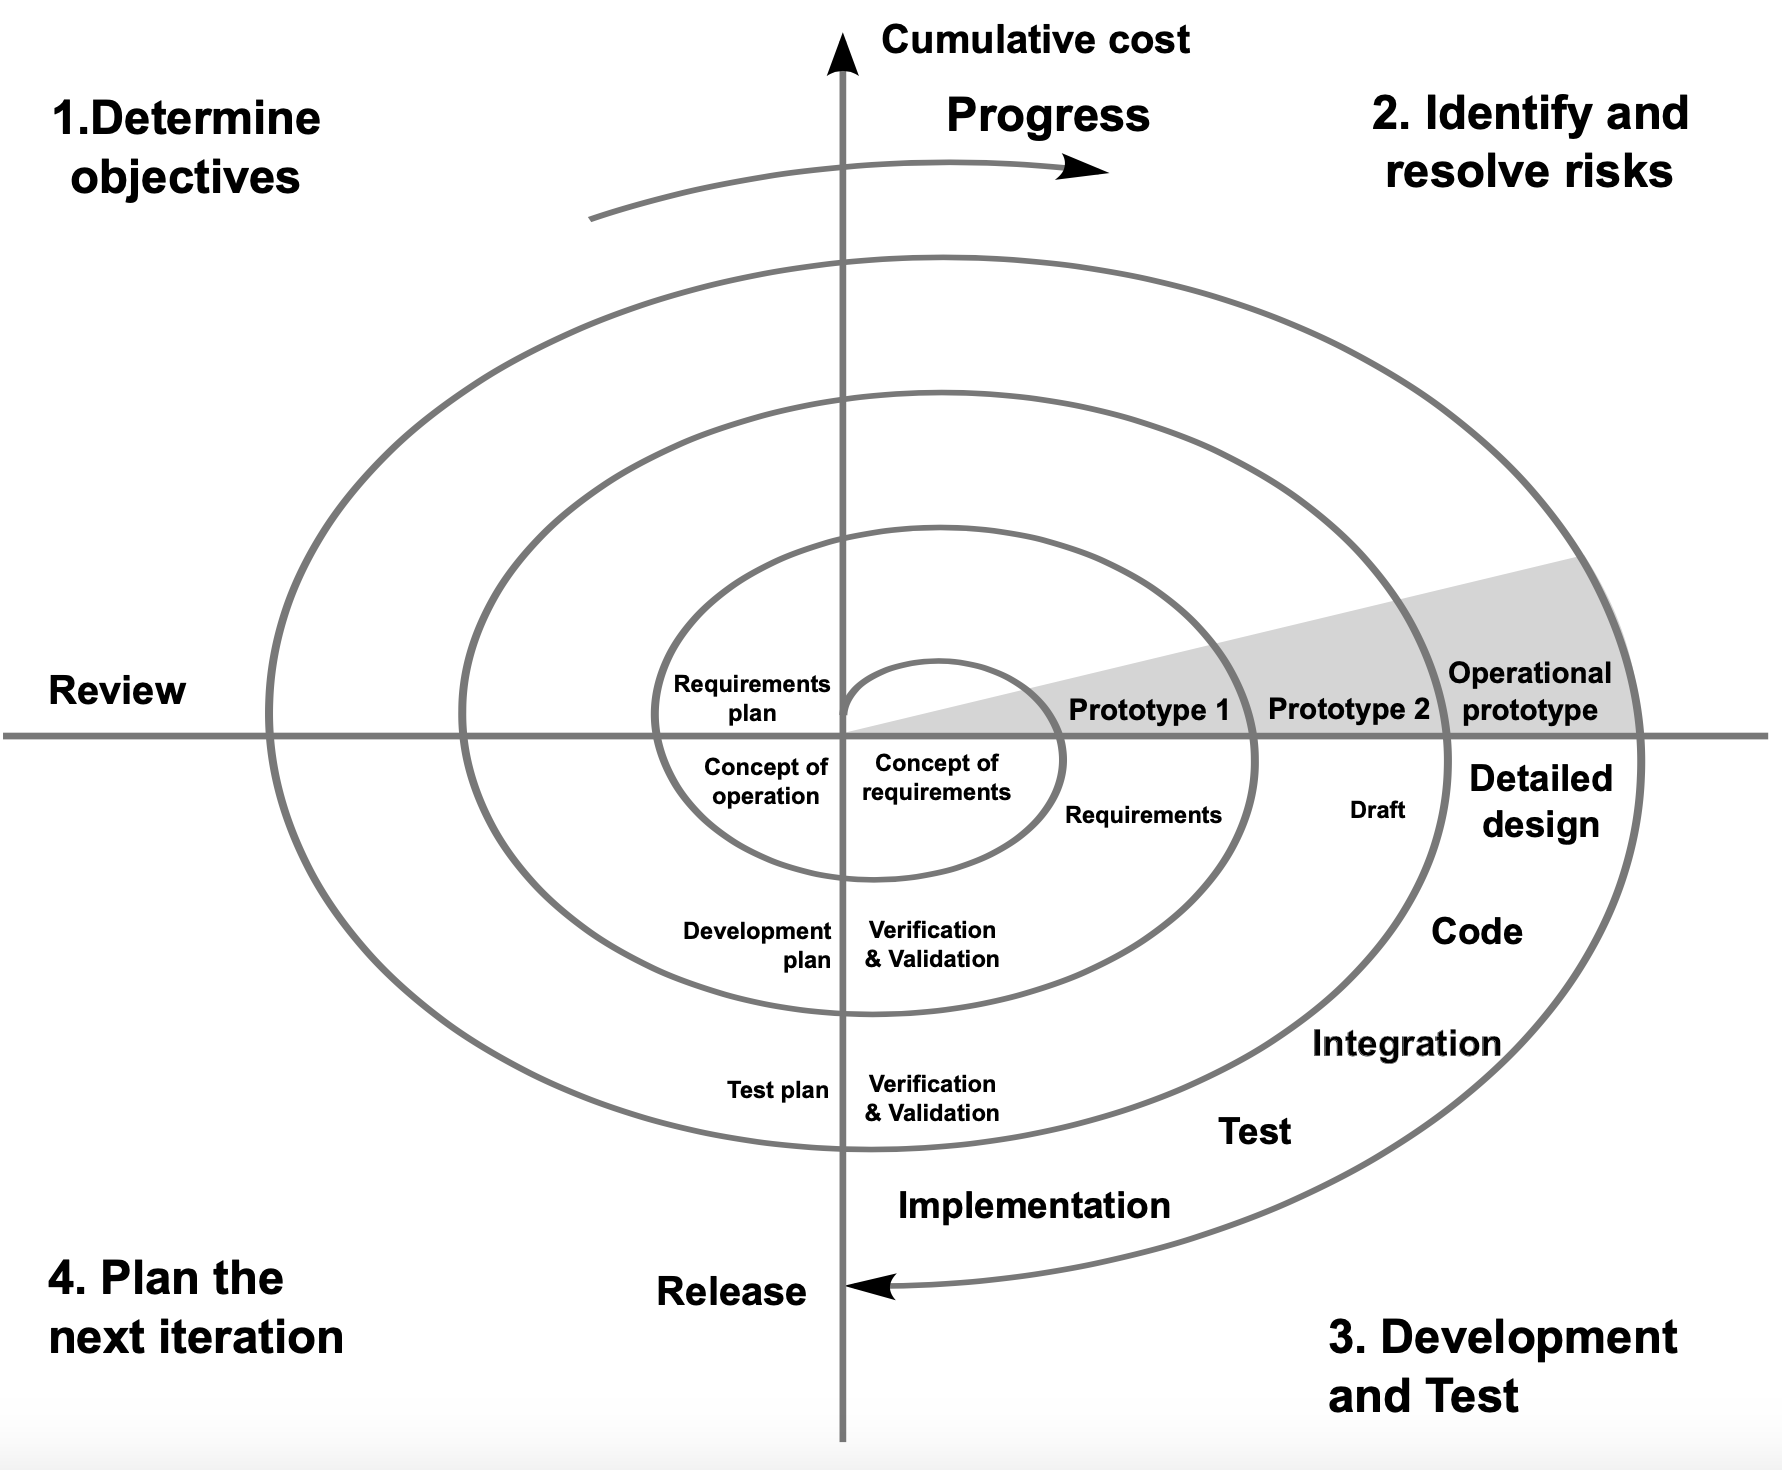
\includegraphics[width=.65\textwidth]{P2023.AIBCCSS.StoryTelling/Spiral_model.png}
    \label{F:Spiral}
\end{figure}


\begin{center}
    \tiny{From: \url{https://en.wikipedia.org/wiki/Spiral\_model\#/media/File:Spiral\_model\_(Boehm,\_1988).svg/}}
\end{center}

\end{frame}


\begin{frame}
{\centerline{More on Rapidity in SW}}

       \begin{tabular}{cl}  
         \begin{tabular}{c}
           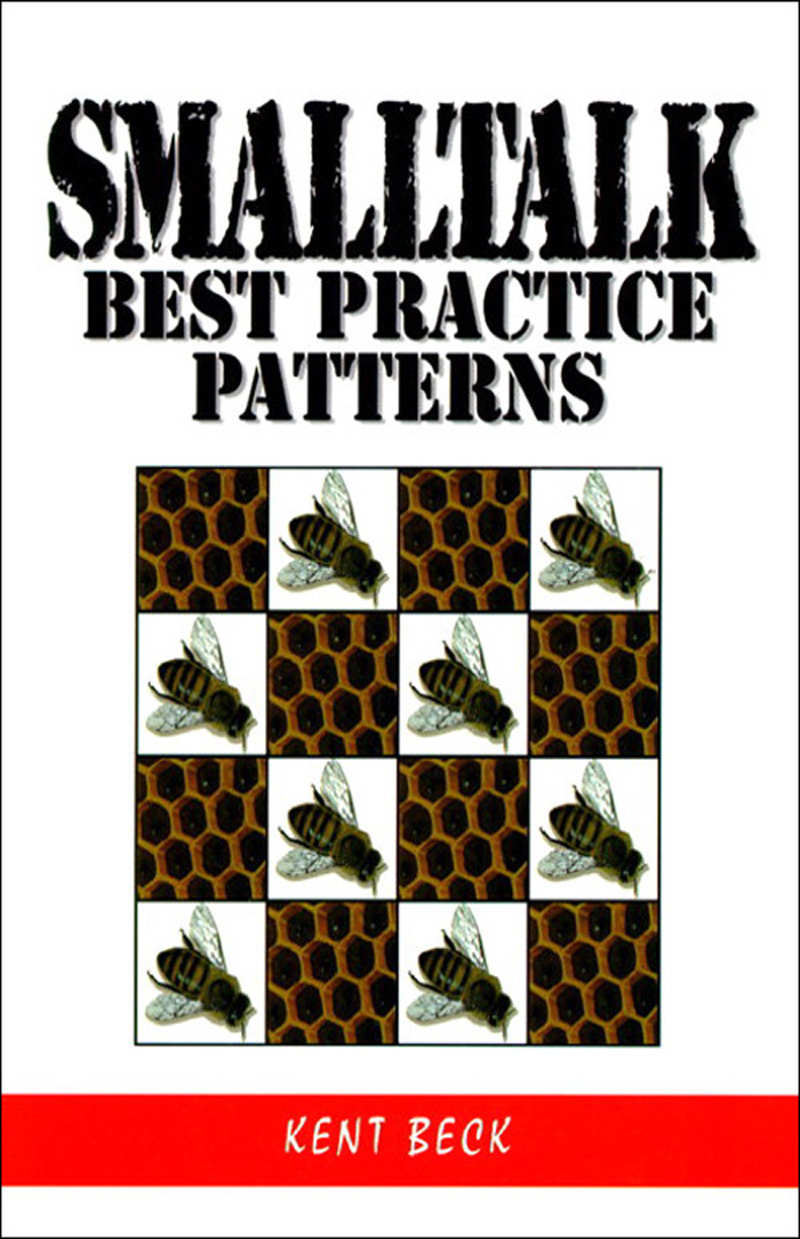
\includegraphics[width=.4\textwidth]{P2023.AIBCCSS.StoryTelling/SmallTalkBeck.jpg}
           \end{tabular}
           & \begin{tabular}{l}
             \parbox{0.5\linewidth}{%  
             \begin{itemize}
                \item ``Do you know that your program talks to you?''
                \item ``\textcolor{cyan}{\textbf{Objects}} (done right) can change all that. Jo longer is your system a slave of representation. Because objects can hide their representation behind a wall of messages, you are free to change representation and only affect one object.''
                \item $\ldots{}$

            \end{itemize}

             }
         \end{tabular}
       \end{tabular}


\end{frame}


\begin{frame}
{\centerline{Rapidity -- New perspectives}}

\begin{itemize}
\item The omission of details is instrumental for interconnecting different parts of a narration without loosing focus \vspace{0.2cm}
\item From Galileo: ``argumenting is like running!''
\begin{itemize}
\item \textcolor{red}{Is it information hiding?} \vspace{0.2cm}
\end{itemize}
\item Repetition to a certain degree is important. 
\begin{itemize}
\item \textcolor{blue}{Could it be assimilated to reuse?}
\end{itemize}

\end{itemize}

\end{frame}

\begin{frame}
{\centerline{Precision}}
\begin{itemize}
\item For Calvino: \vspace{0.3cm}
\begin{itemize}
\item a \textcolor{red}{\textbf{well defined}}  and \textcolor{blue}{\textbf{well planned}} design of a work \vspace{0.3cm}

\item a collection of images that are \textcolor{red}{\textbf{clean}}, \textcolor{blue}{\textbf{crisp}}, \textcolor{orange}{\textbf{easy to memorize}}, \textcolor{cyan}{\textbf{vivid}} \vspace{0.3cm}

\item a \textcolor{red}{\textbf{maximally precise language}}, both in terms of \textcolor{blue}{\textbf{usage of the words}} and  \textcolor{orange}{\textbf{ability to render}}  thoughts and imaginations.
\end{itemize}
\end{itemize}

\end{frame}

\begin{frame}
{\centerline{Quest for Precision}}
\begin{tcolorbox}[fonttitle=\bfseries,nobeforeafter,center title,colback=yellow!5,colframe=yellow!40!black,title=The Plague (for Calvino)]
    ``Often it appears that a pestilential epidemic has plagued the humankind in the aspect that characterizes it the most: the use of the word, a pest of the language that manifests itself as \textcolor{red}{\textbf{loss of cognitive strength}} and of spontaneity, as an \textcolor{blue}{\textbf{automation of forms}} that tend to level expressions toward more generic, anonymous, and abstract formulations, to smooth down crisp expressions, to turn off any sparkle arising when old words occurs in new circumstances."
\end{tcolorbox}

\end{frame}

\begin{frame}
{\centerline{Quest for Precision}}
\begin{tcolorbox}[fonttitle=\bfseries,nobeforeafter,center title,colback=yellow!5,colframe=yellow!40!black,title=The Plague (for Calvino)]
    ``I do not care here whether the root of this epidemic are in politics, in ideology, in the bureaucratic uniformity, in the homogenisation of mass-media, in the scholastic diffusion of middle education. What I am caring about are the possibility of healing. The \textcolor{red}{\textbf{literature}} (and \textcolor{blue}{\textbf{perhaps only the literature}}) can create the antibodies that may contrast such pest of the language."
\end{tcolorbox}

\end{frame}

\begin{frame}
{\centerline{Precision is not completeness}}
\begin{itemize}
\item Writing has to satisfy two, apparently divergent, constraints:
\begin{itemize}
\item on one side, the \textcolor{red}{adherence to a model} based on the story to narrate,
\item on the other side, the ability to \textcolor{blue}{express in limited space} such complexity, without compromising the precision.
\end{itemize} \vspace{0.2cm}
\item The solution for this dilemma is \textcolor{red}{not to ``fill pages with words''} in a humongous effort to put in places all such details, \begin{itemize}
\item rather to separate what is \textcolor{red}{expressed with words} and what is \textcolor{blue}{expressed with omissions}.
\end{itemize}
\end{itemize}

\end{frame}


\begin{frame}
{\centerline{Precision in SW}}
\begin{itemize}
\item The plague (our anecdotal experience):
\begin{itemize}
	\item \textcolor{red}{Alleged senior professionals} claiming to know Android, simply because they could write apps using an IDE, but still not understanding, for instance, that layouts are objects created by reflection through dependency injection
	\item \textcolor{blue}{Self promoted high profile data scientists} able to create models through Kera but unable to explain with proper argumentation the architecture of the network and the values of the associated hyperparameters
	\item \textcolor{brown}{Googling-programmers} searching and copying code from the web without understanding anything of it
\end{itemize}
\end{itemize}

\end{frame}

\begin{frame}
{\centerline{The plague (cont.) }}
\begin{itemize}
	\item \textcolor{orange}{Agile gurus}: self-proclaimed expert  without any thorough understanding of the essence of agile, just replicating as parrots terms and prescriptions -- \textcolor{cyan}{refer to our presentation of 8 years ago here on the Dark Side of Agile}
\end{itemize}
\begin{figure}[htp]
    \centering
     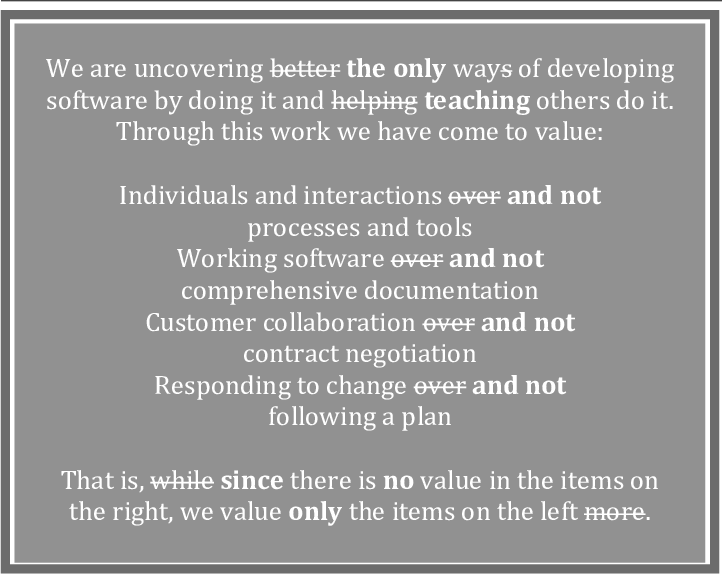
\includegraphics[width=.55\textwidth]{P2023.AIBCCSS.StoryTelling/TheDarkAgileManifesto.png}
    \label{F:TheDarkAgileManifesto}
\end{figure}

\end{frame}


\begin{frame}
{\centerline{Quest for Precision in SW}}
\begin{figure}[htp]
    \centering
     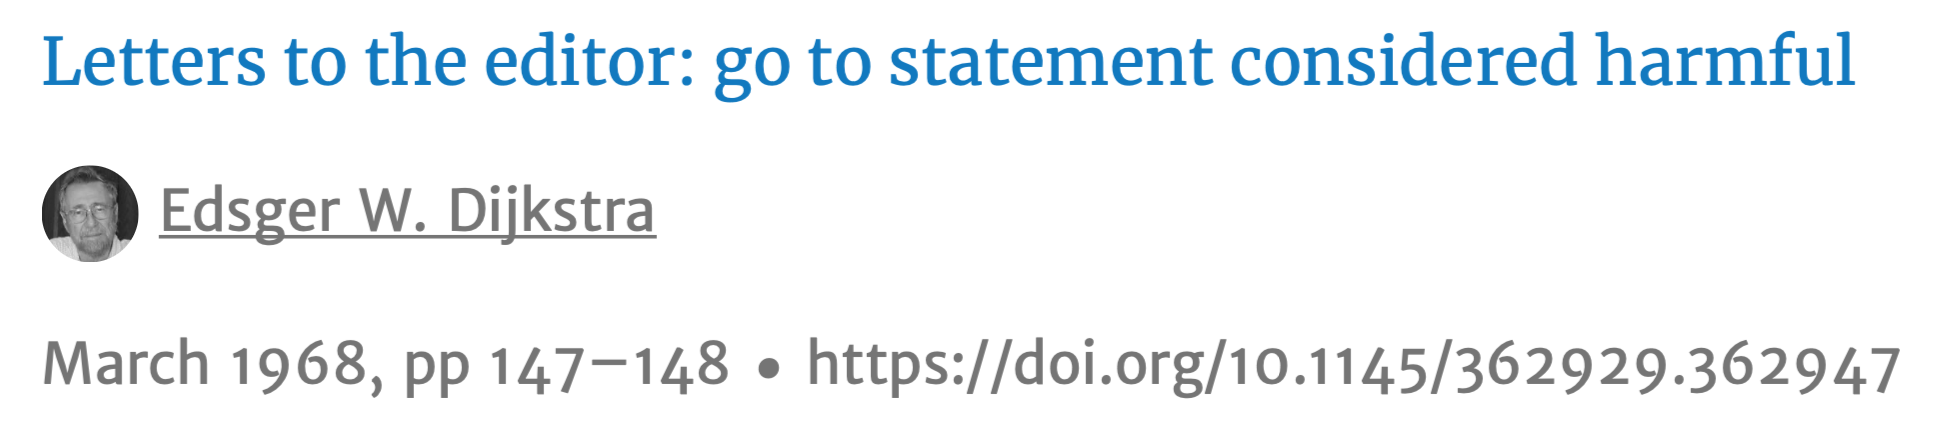
\includegraphics[width=.95\textwidth]{P2023.AIBCCSS.StoryTelling/GoToConsideredHarmful.png}
    \label{F:GoToConsideredHarmful}
\end{figure}
\vspace{-0.1cm}

\begin{itemize}
\item There have been several attempts in the quest to precision:
\begin{itemize}
\item Dijkstra on ``goto considered harmful''
\item Backus on Von Neumann style
\item Turner on indentation
\item Kay on Smalltalk
\end{itemize}
\end{itemize}



\end{frame}

\begin{frame}
{\centerline{Quest for Precision in SW}}
\begin{figure}[htp]
    \centering
     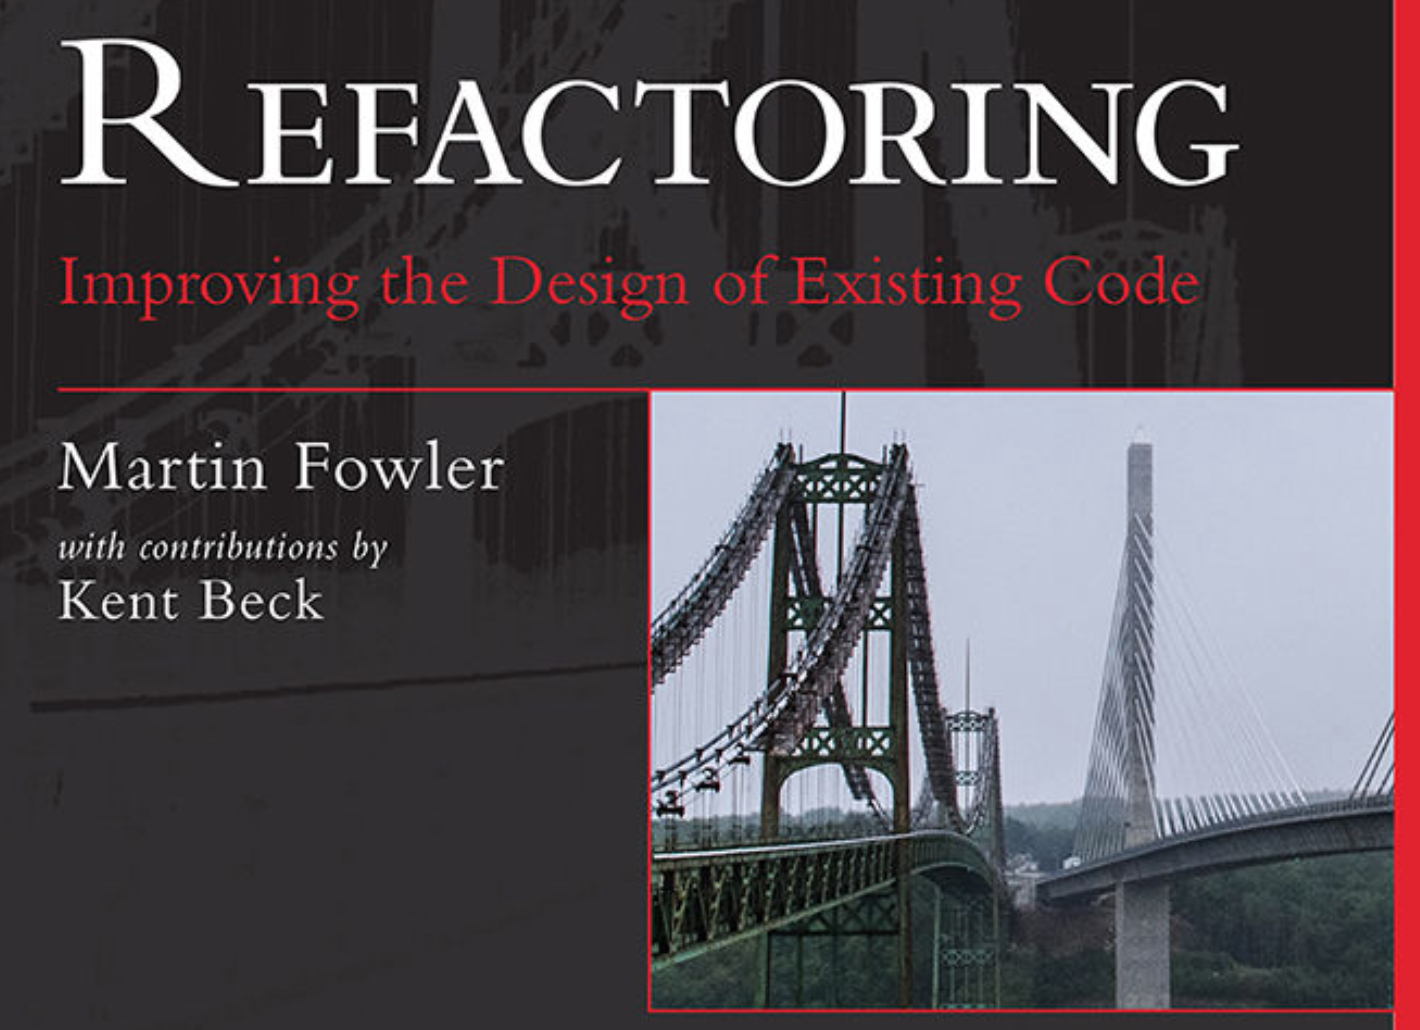
\includegraphics[width=.55\textwidth]{P2023.AIBCCSS.StoryTelling/Refactoring.png}
    \label{F:Refactoring}
\end{figure}
\vspace{-0.1cm}

\begin{itemize}
\item Agile with all its practices, e.g., effective design, simplicity,  refactoring, technical excellence, reflections, $\ldots{}$
\item We should think at an addendum to the Agile Manifesto claiming that \textcolor{red}{Agility (and perhaps only agility) can create the antibodies that may contrast such pest of the language.}
\end{itemize}



\end{frame}


\begin{frame}
{\centerline{Precision -- New perspectives}}
\begin{tcolorbox}[fonttitle=\bfseries,nobeforeafter,center title,colback=yellow!5,colframe=yellow!40!black,title=Impossibility to Generalize]
In reality, always my writing has found itself in front of \textcolor{red}{two divergent ways that correspond to two different kinds of knowledge}: \textcolor{blue}{one that moves itself in the mental space of unbundled rationality}, where we can draw lines that interconnect points, projections, abstract forms, vector of forces; \textcolor{orange}{the other that moves itself in a space full of objects} and tries to create an equivalent verbal of the space filling pages with words $\ldots{}$ They are \textcolor{cyan}{two different compulsions toward precision that will never arrive to the absolute satisfaction} $\ldots{}$ I oscillate continuously between these two ways and when I feel to have completely explored the possibility of one I jump to the other, and viceversa. 
\end{tcolorbox}

\end{frame}

\begin{frame}
{\centerline{Precision -- New perspectives}}
\begin{itemize}
\item Vagueness has a  positive connotation for many poets;
\begin{itemize}
\item because it allows to \textcolor{red}{perceive with a high level of precision} \textcolor{red}{the indetermination} (notice the oxymoron)  of several situations
\item G. Leopardi: ``To this pleasure contributes the variety,  \textcolor{red}{the uncertainty}, the fact that we cannot see everything, and so  \textcolor{blue}{we can elaborate with our imagination what we cannot see}.''
\end{itemize}
\item Usually, it generates a negative feeling while writing software, but what about:
\begin{itemize}
\item variables with names \texttt{i} or \texttt{j}
\item overloading of names
\item overriding of names
\item $\ldots{}$
\end{itemize}
\end{itemize}

\end{frame}


\begin{frame}
{\centerline{Precision -- New perspectives}}
\begin{itemize}
\item A related concept is the appreciation of the \textcolor{red}{impossibility of generalizing}
\begin{itemize}
\item there are situations that appear to be absolutely unique
\item R. Musil: ``There are mathematical problems for which  \textcolor{red}{a general solution does not exist} but rather individual solutions, that, together, approach the general solution.''
\item G. Flaubert `` \textcolor{blue}{The good Lord is in the details}.''
\end{itemize}
\item Being specific is essential to avoid the temptation of generalizing and abstracting
\item The poet should describe one facet of a crystal representing the reality, where every side of the crystal provides a different and complementary views of it.
\begin{itemize}
\item This resonates a bit with agile but it is a concept with potentials still to express.
\end{itemize}
\end{itemize}

\end{frame}

\begin{frame}
{\centerline{Visibility}}

\begin{tcolorbox}[fonttitle=\bfseries,nobeforeafter,center title,colback=yellow!5,colframe=yellow!40!black,title=Vision]
The process by which the fantasy elaborates images of sensations and feelings. What happens when Dante says: ``\textcolor{red}{It rained inside the high fantasy}.'' and ``\textcolor{blue}{Oh imagination, you who capture our attention so strongly that even 1000 trumpets could not distract us from you, who move moves you even when what our senses do not instruct you?}'' 
\end{tcolorbox}

\begin{itemize}
\item Visibility plays a dual role in understanding:
\begin{itemize}
\item when we provide a visual representation of the reality;
\item  when we see an image and we reconstruct the reality in a verbal form.
\end{itemize}
\end{itemize}

\end{frame}

\begin{frame}
{\centerline{Visibility}}

\begin{itemize}
    \item Images are often generated telling stories and 
    \begin{itemize}
    \item stories are generated from images.
    \end{itemize}
    \item The narration is:
\begin{itemize}
    \item a tool \textcolor{red}{to understand},
    \item and a way \textcolor{blue}{to provide additional insights} and ask for an additional understanding,
    \item but importantly  also as a \textcolor{orange}{collection of possible hypotheses of what could be}.
\end{itemize}
\item Images will evolve:
\begin{itemize}
    \item being \textcolor{cyan}{standardized}
    \item \textcolor{red}{revising completely the creation process}, especially for new and more challenging tasks.
\end{itemize}
\end{itemize}

\end{frame}

\begin{frame}
{\centerline{Visibility in SW}}

\begin{figure}[htp]
    \centering
     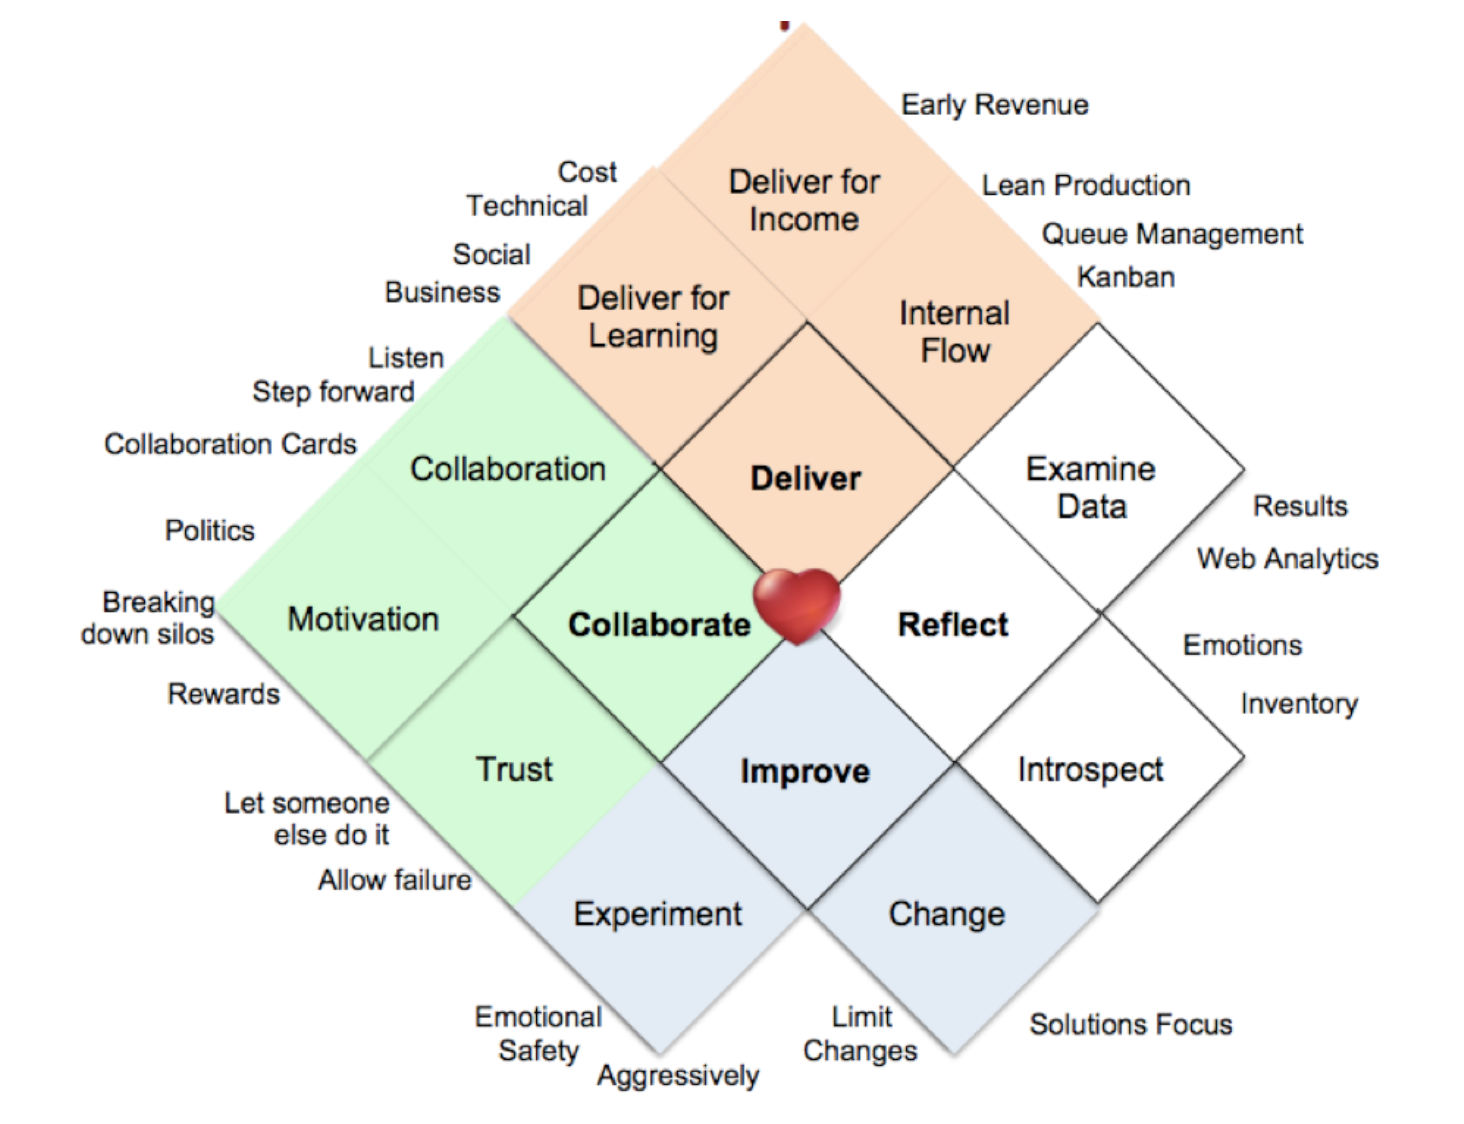
\includegraphics[width=.68\textwidth]{P2023.AIBCCSS.StoryTelling/HeartOfAgile.png}
    \label{F:HeartOfAgile}
\end{figure}
\vspace{-0.2cm}

\begin{center}
``\textcolor{blue}{Oh imagination, you who capture our attention so strongly $\ldots{}$}'' \\
\tiny{From: Alistair Cockburn \textit{The Heart of Agile}
 \url{https://alistair.cockburn.us/wp-content/uploads/2018/02/The-Heart-of-Agile-Technical-Report.pdf}}

\end{center}

\end{frame}


\begin{frame}
{\centerline{Visibility in SW}}

\begin{itemize}
    \item The approach by Calvino/Dante is a \textit{de-facto} standard
    \item The dual role of visibility in understanding occurs in several parts of the development process -- \textcolor{red}{roundtrip engineering}
    \item Visibility facilitates agility through the creation of vivid images of what we are developing:
    \begin{itemize}
    \item consider the example of \textcolor{blue}{metaphors}
    \end{itemize}
    \item Narration has exactly the same role for visibility
    \item Also the future of images appears to resonate:
    \begin{itemize}
    \item We are spectators of the process of standardizing images
    \item In several fields we see a restart of the process of generating images, e.g., in dashboarding, business analytics, etc.
    \end{itemize}
\end{itemize}

\end{frame}

\begin{frame}
{\centerline{Visibility -- New perspectives}}
\begin{itemize}
\item Calvino outlines two possible interpretations of the process of building representations of the world:
\begin{itemize}
    \item \textcolor{red}{as communication of internal state of minds}
    \item \textcolor{blue}{as emergence of knowledge archetypes} 
\end{itemize}
These concepts are practically new in writing SW but they appear to have strong potentials. \vspace{0.3cm}
\item Calvino promotes a pedagogy of imagination that could be very relevant for SW writers.

\end{itemize}

\end{frame}

\begin{frame}
{\centerline{Multiplicity}}
\begin{tcolorbox}[fonttitle=\bfseries,nobeforeafter,center title,colback=yellow!5,colframe=yellow!40!black,title=Ambition of Literature]
Excessive ambitions can be blamed in many areas of human endeavours, but not in literature. \textcolor{red}{The literature lives only if it sets humongous objective's}, even beyond what is conceivable. Only if poets and writers will aim at achieving enterprises that  none else even dare to dream the literature will continue to have a purpose. At the time at which the science is wary of general explanations and of solutions that are not sectorial and specialized, \textcolor{blue}{the big challenge for literature is to be able to weave together the different knowledge and the different codes within a plural and multifaceted view of the world.}
\end{tcolorbox}

\end{frame}

\begin{frame}
{\centerline{Multiplicity}}
\begin{itemize}
    \item There a set of \textcolor{red}{features that appears constants} throughout years and styles
    \item About the \textcolor{blue}{amount of information}:
    \begin{itemize}
        \item there is a tendency of provide a plenitude of details, and
        \item there is an approach to minimize the possible information flow 
    \end{itemize}
    \item There is a large amount of \textcolor{orange}{writers that did not complete (some of) their works}, e.g., Virgilio (Latin, 70BC-20BC), Dante (Italian, 1265-1321), Goethe (German, 1748-1832), Proust (French, 1871-1922), $\ldots{}$
    \item Books tend to have a \textcolor{cyan}{life well beyond the one originally thought by the author} -- see for instance the case of Harry Potter

\end{itemize}   
\end{frame}

\begin{frame}
{\centerline{Multiplicity}}
\begin{itemize}
    \item Four classes, wrt multiplicity:
    \begin{itemize}
        \item texts following a \textcolor{red}{single inspiration, but that can then be understood at multiple levels};
        \item works where \textcolor{blue}{multiple narrations} intersect strongly within a well defined context, but without providing an overall unifying vision;
        \item  attempts to create a \textcolor{orange}{single and unifying vision} of the whole work, that then is very likely to never be completed;
        \item collections of \textcolor{cyan}{non contradictory aphorisms}, which do not give a comprehensive and explicit view of the subject of discussion, but shed lights on aspects of it
    \end{itemize}

\end{itemize}   
\end{frame}

\begin{frame}
{\centerline{Multiplicity in SW}}
\begin{itemize}
    \item Also in SW there are:
    \begin{itemize}
        \item  methods that attempt to create comprehensive models of the systems to develop;
        \item  alternative ideas that software should be minimalistically designed. 
    \end{itemize}
    \item Especially when developed using waterfalls, software development exhibits the natural tendency of never ending
    \item Software is also exposed at the expansion of its original intention well beyond the initial ideas, as it is evident for instance in the history of PowerPoint
\end{itemize}   
\end{frame}


\begin{frame}
{\centerline{Multiplicity in SW}}
\begin{itemize}
    \item The four classes exist (with modification):
    \begin{itemize}
        \item \textcolor{red}{single inspiration but multiple interpretations}: this reflects the idea of describing a system as a set of different and coherent views, as it was done, for instance, in the mid-90s with the methodologies developed around the newly defined UML;
        \item \textcolor{blue}{multiple narrations} proceeding in parallel: this appears to be quite present in agent-based systems;
        \item \textcolor{orange}{single and universal description}: this is what happens when we try to build an omni-comprehensive system;
        \item collection of \textcolor{cyan}{non contradictory simple models}: this resembles strongly agile methods collecting requirements in the forms of simple users stories and then developing incrementally.
    \end{itemize}

\end{itemize}   
\end{frame}

\begin{frame}
{\centerline{Multiplicity -- New perspectives}}
\begin{itemize}
    \item ``\textcolor{red}{hyper-romance}'', that is a romance that is a combination of multiple plots, also with multiple starting or ending points
    \begin{itemize}
        \item interesting reference point for what we have in software as \textcolor{red}{frameworks} for creating different applications
    \end{itemize} \vspace{0.2cm}
    \item the \textcolor{blue}{romance as a network of ideas}, and even of \textcolor{orange}{contributions from different people}, like an \textcolor{cyan}{emerging entity}
    \begin{itemize}
        \item open source communities have created software based on \textcolor{orange}{various contributions of different
        people}
        \item agile methods have emphasized the concept of \textcolor{cyan}{emerging architectures}
    \end{itemize}
\end{itemize}   
\end{frame}

\begin{frame}
{\centerline{Conclusions -- Some important takeaways}}
\begin{itemize}
\item Description by under-specification and by vagueness
\begin{itemize}
\item consider also random gradient descend
\end{itemize}  
\item Rapidity in writing, certain activities cannot be performed slowly
\item Generalizing is intrinsically a bogus process
\item Creations of visual models and of metaphors
\item Narrations are like live entities
\end{itemize}   
\end{frame}


\begin{frame}
{\centerline{Questions?}}

\vspace{1cm}
\begin{center}
    \LARGE{End of lecture nine.}
\end{center}

\end{frame}


\end{document}
